Transitioning to a computational model provided us with the tools necessary to explore larger systems and gave us greater control over the individual cell action potentials. With the goal to create a lightweight model that effectively models the action potential of each cell; we committed to using a FN equation to model each individual cell in a homogeneous cubic lattice. This ignores the anisotropy in the biological system but dramatically reduces the computational cost. \par

The lack of anisotropy is justified as the model is designed to simulate a small section of right atrial tissue. In tissue, on this scale, the fibre structure that causes the anisotropy is heavily interconnected so can largely be ignored. When scaling up, this anisotropy could be easily included by applying a matrix to the equation which acts as a tensor. This tensor could be as simple as a scalar factor applied in each different direction of propagation or more complex to include further geometric effects. \par
The full commented code can be found in the appendix \ref{appendix2D}.

\subsection{FN Model of an Isolated Cell}
\label{sectionisocell}
Our computational model uses a FN equation based on the three transistor circuit model as described in section \ref{section3} \citep{3transistor}. Each cell's action potential ($u$) is controlled by a gating variable $v$ with the parameters $a$, $b$ and $\epsilon$ controlling the shape of the action potential curve. The initial activation potential is a function of time, $t$, as $s(t)$. The equationss take the form of
\begin{equation}
    \begin{split}
        & \frac{du}{dt}=u(u-a)(1-u)-v+s(t) \\
        & \frac{dv}{dt}=\epsilon (u-bv)
    \end{split}
    \label{eqmodel}
\end{equation}
and $u$ is plotted against $t$ to give the action potential. For the initial cell (the simulated SAN) the parameters $a, b$ and $\epsilon$ are given the values 0.15, 2.5 and 0.01 respectively. Also to simulate the external driving force that triggers the heart beat the $s(t)$ term is given a value of 0.06 for a small pulse duration (5 dimensionless time units). These parameters create an action potential as shown in figure \ref{fig5.2b}. This action potential is very similar to the action potential seen in SAN cells and as such will be used as the initial cell's action potential in our full model. \par

All values are dimensionless but an estimate of their equivalent values can be made using the multiplication factors in table \ref{tabdimensionless}. It is also important to note that dimensionless time, $t$, is sampled in steps. The sample rate set in these simulations is set at a value of 6, meaning that each dimensionless time unit is made up of 6 individual time 'steps'.

\begin{table}[H]
    \centering
    \begin{tabular}{||c c c||} 
 \hline
 Cell & membrane potential (mV) & t (s) \\ [0.5ex] 
 \hline\hline
 SAN & $(u\times94.4\pm 2)-55$ & $\times1.2\pm 0.3$\\ 
 \hline
 Atrial & $(u\times67.0\pm 2)-80$ & $\times0.5\pm 0.15$\\
 \hline
    \end{tabular}
    \caption{Multiplication factors to estimate equivalent values of the membrane potential and time from the model output.}
    \label{tabdimensionless}
\end{table}

\subsection{Propagation Mechanism}
To propagate the signal through the medium and simulate the travelling wavefront we must create a method of activating neighbouring cells. To do this we create a homogeneous cubic lattice of cells where each cell checks its nearest neighbours action potential, $u$, after a delay time, $d$, which represents the diffusion time of the extracellular ions between cells. This delayed potential of the first cell becomes the activation potential ($s(t)$) of the second. As such, the second cell's equations relative to the first can be described as
\begin{equation}
    \begin{split}
        & \frac{du_2}{dt}=u_2(u_2-a)(1-u_2)-v_2+u_1(t-d) \\
        & \frac{dv_2}{dt}=\epsilon(u_2-bv_2)
    \end{split}
\end{equation}
were $u_2$ is the action potential of the second cell and $u_1(t-d)$ is the action potential of the first cell at time $t-d$. \par

When the previous cell's action potential is passed on in this way to the next (with the same parameters as indicated in section \ref{sectionisocell}) the action potential becomes more like a square wave. This is shown in figure \ref{fig5.2b} and is very similar in shape to an atrial cells action potential. This is then propagated in a similar way across the full geometry.

\begin{figure}[H]
    \centering
    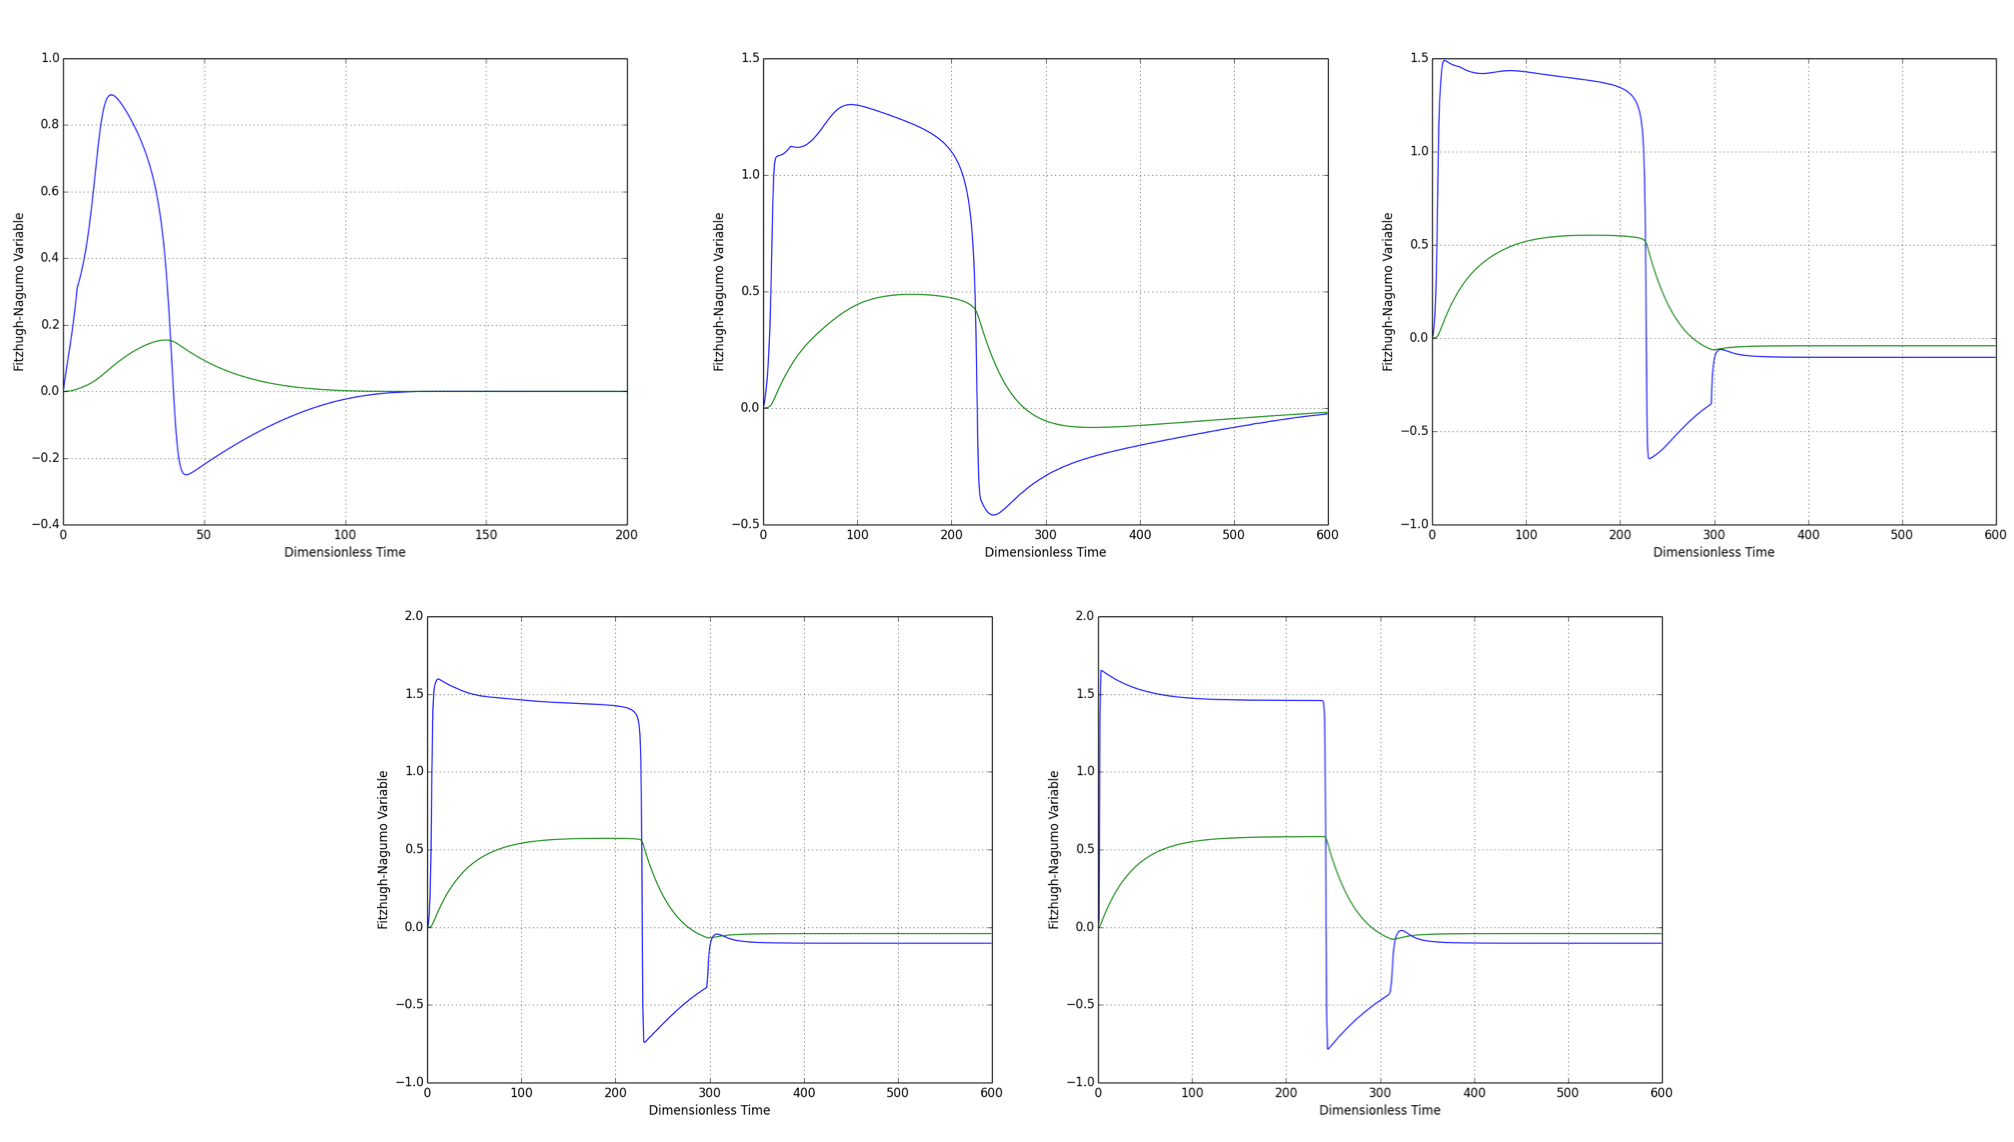
\includegraphics[width=\textwidth]{images/cellpotentials.png}
    \caption{Membrane potential outputs for a SAN cell, a $1^{st}$ column cell, a $2^{nd}$ column cell, a $3^{rd}$ column cell and a $30^{th}$ column cell (top left to bottom right). The blue and green lines show the membrane potential and gating variable respectively. The SAN output is very similar to a typical SAN cell membrane potential as shown in figure \ref{fig2.6}. The output then morphs into more of a square wave potential which can be used to model the atrial cells with the output resembling an exaggerated version of figure \ref{fig2.5}.}
    \label{fig5.2b}
\end{figure}

\subsection{2D Simulation}
In two dimensions on a 81 by 81 grid of cells, a simulation over 1800 dimensionless time units takes approximately 2 hours on a single thread of a 2.4Ghz Intel i5 processor. The code could be adapted for multi-threading and larger more complex geometries used, however, for proof of concept and functionality all following 2D simulations are carried out with these parameters. A tool for graphically displaying the output binary files can be found in appendix \ref{appendix2D}.\par

For a single beat across the geometry the first column of the matrix (x-coordinate equal to zero) is given an excitation pulse of 0.06, as described in section \ref{sectionisocell}, to simulate SAN activation. This can be expanded further to allow multiple beats as shown in figure \ref{fig5.3a}. \par
\begin{figure}[H]
    \centering
    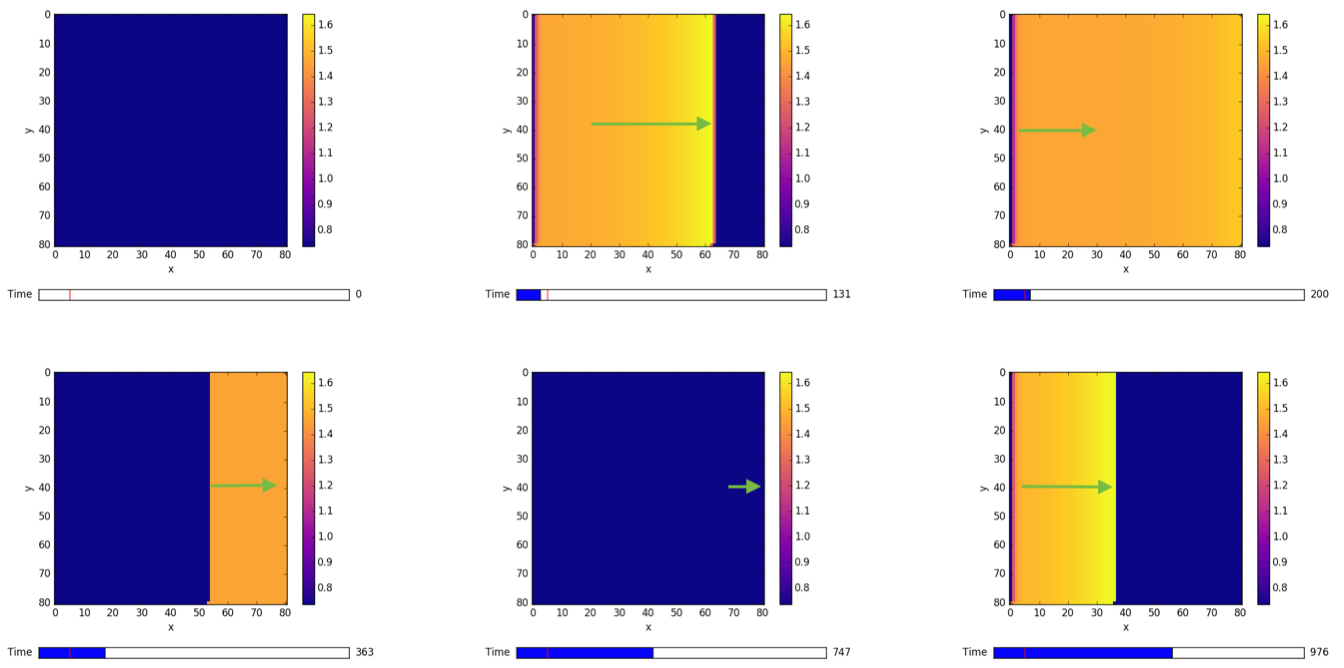
\includegraphics[width=\textwidth]{images/2beatimage.png}
    \caption{A two beat simulation with the parameters detailed in section \ref{sectionisocell}. The $x=0$ column was used as the SAN and given an initial excitation pulse of 0.06 for 5 dimensionless time units, the first at $0\leq t \geq 5$ and the second at $150 \leq t \geq 155$. The sample rate (effectively the diffusion time) is 6. The green arrows show the wavefront propagation direction. It is clear that the wavefront travels uniformly and the system relaxes as expected ready for sequential excitations.}
    \label{fig5.3a}
\end{figure}

    \subsubsection{Re-entrant Tachycardia}
    One of the causes of re-entrant tachycardia is the presence of a uni-directional blocker as described in section \ref{section2.4}. Uni-direction blockers can be simulated in our model. A uni-directional blocker blocks propagation in the positive $x$ direction but allows propagation in the negative $x$ direction. This can delay the signal for long enough to allow cells to relax and re-excite as shown in figure \ref{fig5.3.1a}. This re-entry can cause spiral waves to occur causing multiple re-excitations and thus a faster heart rate. \par
    \begin{figure}[H]
        \centering
        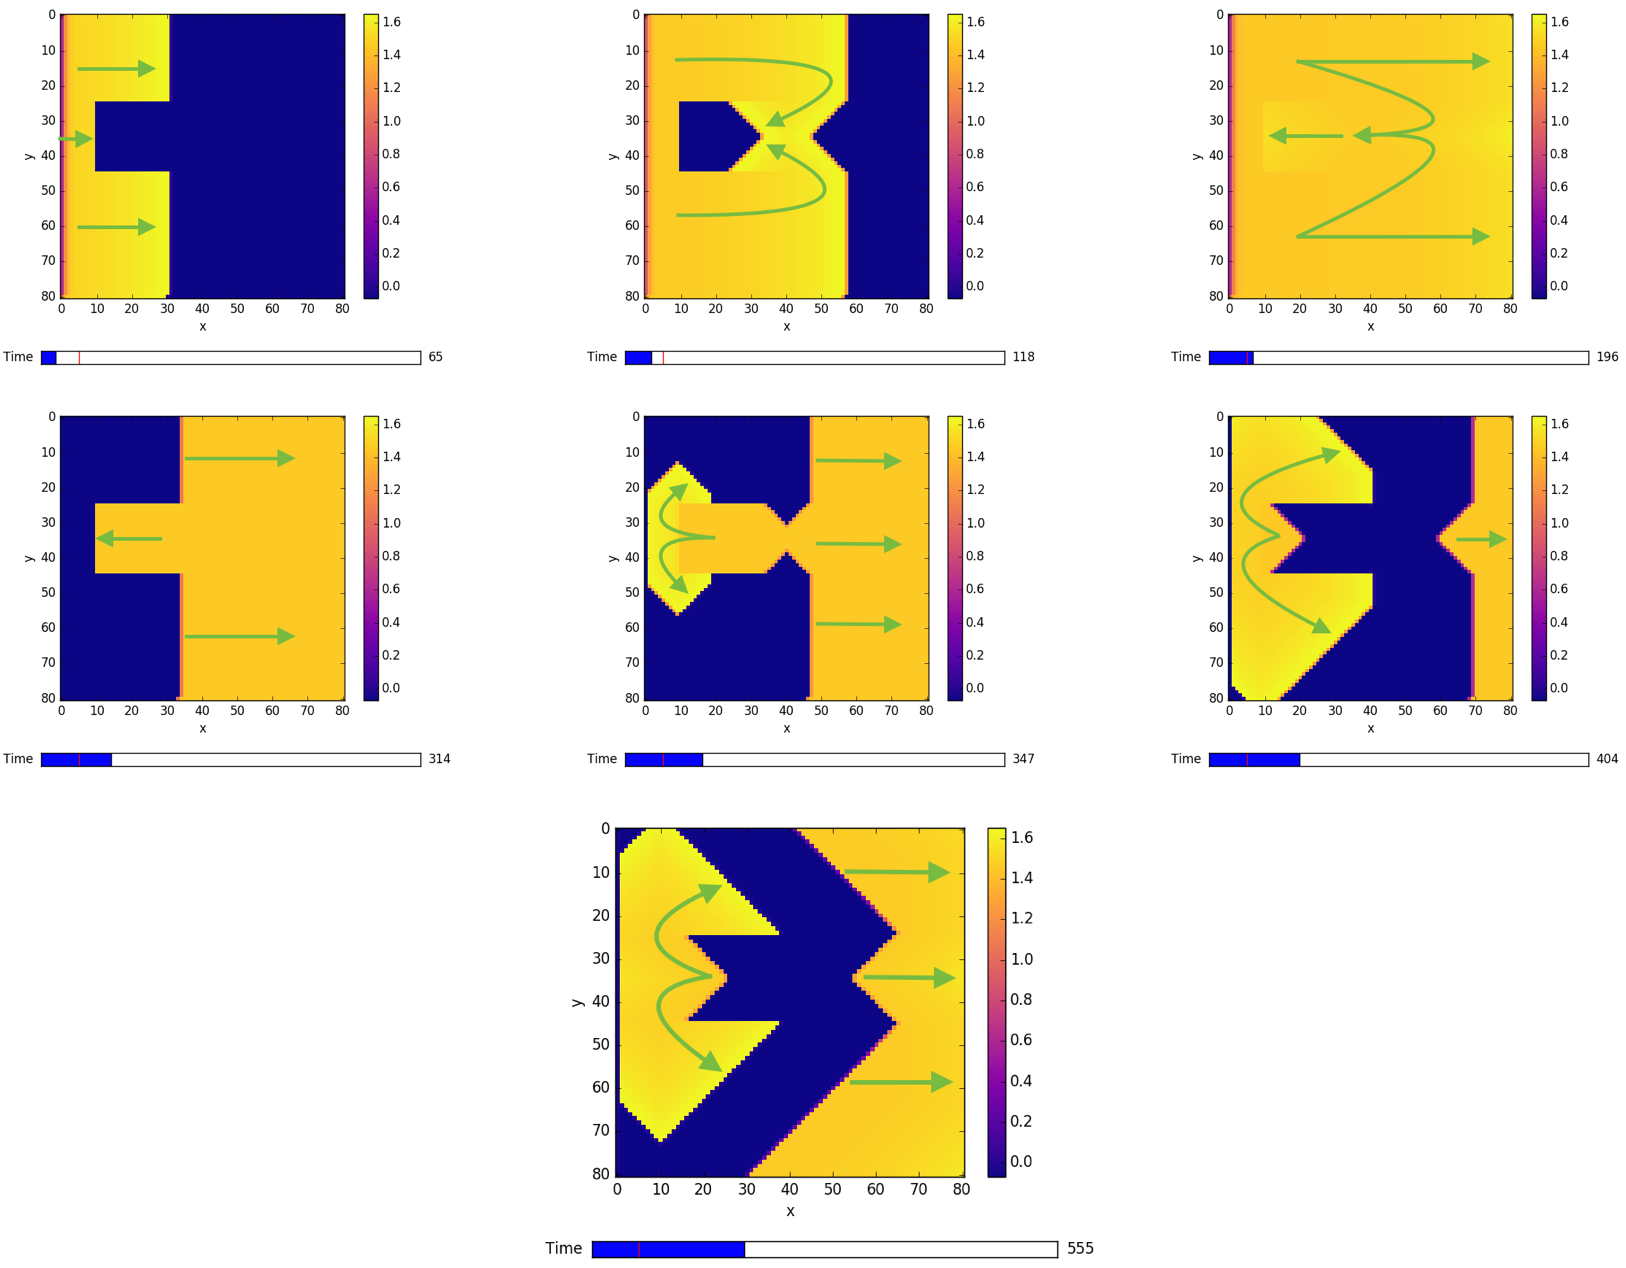
\includegraphics[width=\textwidth]{images/uniblocker.png}
        \caption{The $x=0$ column was used as the SAN and given an initial excitation pulse of 0.06 for 5 dimensionless time units at $t=0$. The sample rate (effectively the diffusion time) is 6. The green arrows show the wavefront propagation direction. The uni-directional block is a rectangle located at (10, 25) to (30, 45). Initial forward propagation is halted at the blocker, the wavefront passes the blocker and propagates back through it in the negative $x$ direction. After a period of time the cells at the forward edge of the blocker relax to a point where they can be re-excited. This allows re-entry and the wave front to re-propagate across the medium. Theses shorter echos cause the whole medium to excite simulating the effects of tachycardia.}
        \label{fig5.3.1a}
    \end{figure}
    
        \subsubsection{Ablation}
        One regularly used treatment for this kind of re-entrant tachycardia is to destroy the tissue of the blocker, effectively transforming the area from a uni-directional blocker to an omni-directional blocker. The surgical way of achieving this is via ablation, \citep{ablation2}. Ablation typically involves the use of a catheter which is used to apply radiofrequecy radiation to the effected area killing the tissue \citep{ablation}. The omni-directional blocker created does not allow backwards (negative $x$ direction) propagation so re-entry does not occur causing an end to the tachycardia.
        \begin{figure}[H]
            \centering
            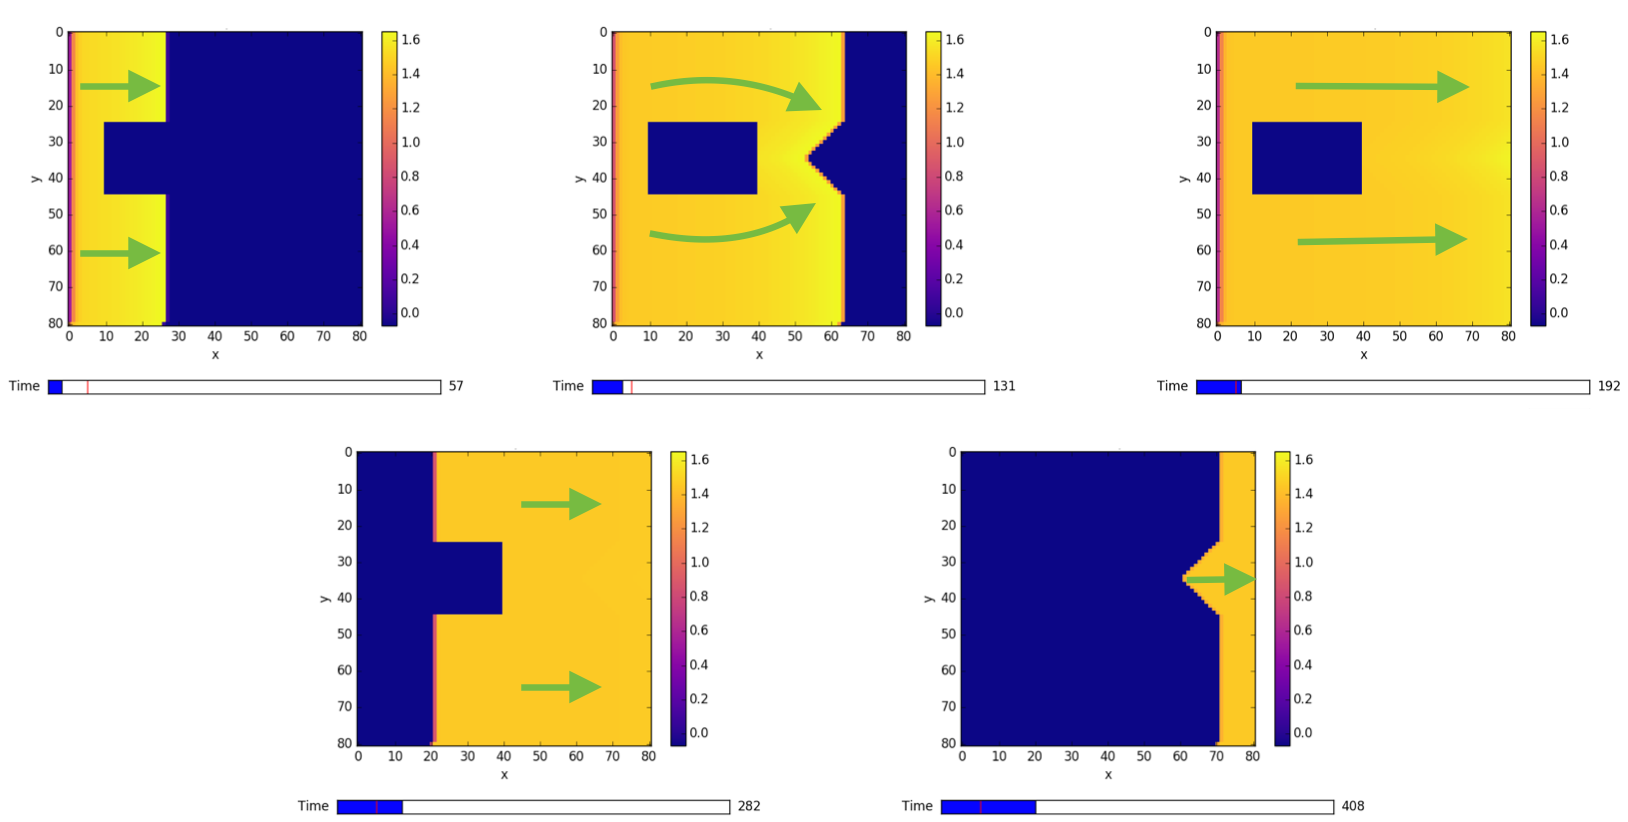
\includegraphics[width=\textwidth]{images/ablationfull.png}
            \caption{The $x=0$ column was used as the SAN and given an initial excitation pulse of 0.06 for 5 dimensionless time units at $t=0$. Sample rate is 6. Green arrows show the wavefront propagation. The omnidirectional block is a rectangle located at (10, 25) to (30, 45). Propagation is stopped in all directions by the blocker so the signal cannot propagate though the region. This does not allow any re-entry effects to occur keeping the beat rate normal.}
            \label{fig5.3.2a}
        \end{figure}

        \subsubsection{Drug Treatment}
        An alternative approach to surgical treatments is a pharmaceutical method to managing arrhythmias. Membrane ion channels and receptors are the key targets of these drugs. As previously identified; the Ca$^{2+}$, K$^+$ and Na$^+$ ion channels are vital in the generation of cardiac action potentials. \par 
        Conduction in the SA and AV nodes is dependent on Ca$^{2+}$ ion channels, therefore, Ca$^{2+}$ channel blocking drugs, such as lacidipine \citep{drugs}, are specific to arrhythmias in these regions. In other regions such as the atrium, the conduction is controlled mostly via the Na$^+$ currents and thus Na$^+$ channel blocking drugs are potentially the most effective agent. Both the Na$^+$ and Ca$^{2+}$ ions contribute to the inward current during the plateau period and as such blocking either channel would prolong the action potential duration potentially preventing re-entry.\par
        The K$^+$ ion channels contribute mainly to the repolarisation phase, as such, blocking these channels can potentially increase the action potential duration and the refractory period. The increased duration and refractory period can prevent cells from being re-excited by re-entrant effects from uni-directional blockers. This is shown in figure \ref{fig5.3.3b} where the effect of a K$^+$ channel blocking drug, such as Amidarone \citep{drugs}, was simulated by reducing the $b$ parameters in equation \ref{eqmodel} to 0.5. This reduces the gating variable's growth rate effectively reducing the repolarisation rate and thus simulating the effect of blocked K$^+$ channels.\par

        \begin{figure}[H]
            \centering
            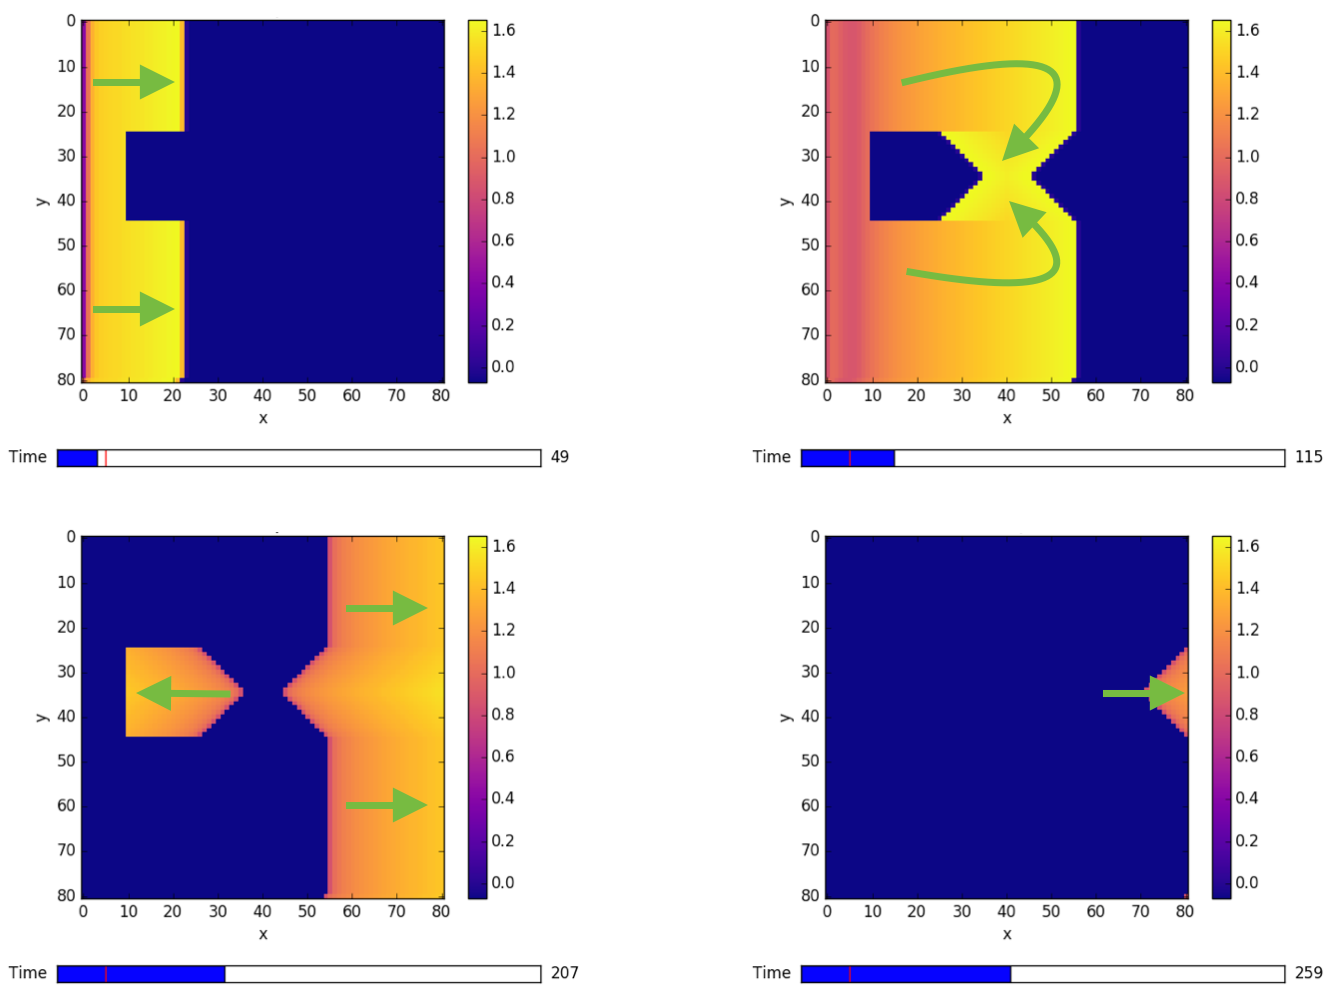
\includegraphics[width=0.8\textwidth]{images/kblock.png}
            \caption{The $x=0$ column was used as the SAN and given an initial excitation pulse of 0.06 for 5 dimensionless time units at $t=0$. Sample rate is 6. Green arrows show the wavefront propagation. Unidirectional block is a rectangle located at $(10, 25)$ to $(30, 45)$. The parameter $b$ is set to 0.5 decreasing the repolarisation phase simulating the effect of K$^+$ ion channel blocking drugs. The wavefront propagates around the unidirectional block and back propagates as before, however, due the the extended refractory period the cells do not re-excite preventing re-entry so no tachycardia is seen.}
            \label{fig5.3.3b}
        \end{figure}
        
        As the simulation is on the cellular level, there is the potential for a more advanced version of this model to be used for novel drug dosing simulation. 
        
\subsection{3D Simulation}
All simulations above have been carried out in a 2D cubic lattice geometry. Due to how the model is constructed it is trivial to add an additional dimension and expand to a 3D geometry. No simulations in 3D space have been included in this document as in a homogeneous lattice the 3$^{rd}$ dimension has very little effect on the outputted heat maps. The 3D system could be used to model more complex geometries, such as hollow ellipsoids, which more accurately represent the geometry of the atrium. A 3D model could also be modified to plot an average atrial potential against time graph, effectively modelling the P wave for comparison with diagnostic ECGs.